

\documentclass{article}

\usepackage{blindtext}
\usepackage{multicol}
\usepackage{array}
\usepackage{float}

\usepackage{geometry}
 \geometry{
 a4paper,
 total={170mm,257mm},
 left=20mm,
 top=20mm,
 }

\usepackage{graphicx}

\title{Tokenomics for a curation DAO}
\author{binderl\\
builderl@laposte.net\\}
\date{\today}

\begin{document}

\pagestyle{myheadings}

\maketitle

\begin{multicols}{2}[]

\begin{abstract}
	Tokenomics science is the way to distribute token to prevent from being scammed. in The Art and Science of Native Token Liquidity from \cite{eva} the author suggests to manage liquidity pool to buy into and to exit. This is obviously a way to follow with big amount of liquidity to ensure exchange rate, no impermanent loss and external attack. In case of low liquidity one way to increase robustness is to pool together. Mining protocol can be used to figure out on those situation. in \cite{qtz:UchArb} a magic button is used to mine in exchange of fees. At the end of the process one miner keep fees of everyone. It's a time game, to get the full reward you need to be the last miner before the next round. In that story miners are monitored they used of the protocol by how much coins they get on wallet. That should be true if the exchange of evidence you get from the protocol are not exchangeable unless if the amount of coins on exchange are less available than the reward you get from the protocol. That lead to think about a mint layer system control by the total value lock to mine. It should be organised in terme of a game to gather maximal attention.

\end{abstract}

\section{Introduction}
Imagine a space in a museum or a stage in a festival, that’s fully curated by the community of the institution. A swarm of DAOs where artists can collaborate, share profit, and build secondary markets with curators, collectors galleries in the metaverse or in real life. A digital space where communities can make themselves heard.

it's assume on this paper this following conception about curation DAOs:
\begin{itemize}
	\item it can be used, organized by anyone without technical knowledge in advance.
   \item Users of the DAO are the only ones responsible for the DAO health.
   \item Users need to act or collaborate to act for getting value. From actions, the DAO are laverage which contribute to increase value.
   \item DAO’s is a space where users can meet each other to decide, play …
   \item DAO is a powerful tools to gamify and power balance. Kind of a new layer with social impact. 
\end{itemize}      
The paper is an introduction on a structural way to leverage the link between making value  and a better DAO Health

\section{DAO - Health}

To be fully curated DAO need to be autonomous. If one part stop acting, the DAO’s continue to do the job until every part quit. This idea is responsible for sustaining the DAO over time. In case of DOS (deny of service) attack over time a DAO need to be resilient. And finally, it should be scalable enough for someone to get what he is looking for.

\subsection{Resilient}

Practically, one things a DAO can do to exist from the view point of the network is to manage to release a contract to explicitly monitor their rules. In that way users can share the American constitution which is divided and represented by a contract. In that case, the amount of tv (total value) on the contract monitor the value of the American constitution. 
The resilience metrics deals with external perturbation. If someone get to enter with half of the share allocated on the contract, he should say i get enough power to do what I want. And also internal because of accumulation over time.
In this conception internal and external perturbation can be monitored with the amount of share which is directly available to exchange.

\emph{To be healthy resilient DAO need to manage their liquidity.}

\subsection{Scalable}
anyone can enter on the DAO without disturbing the whole. It is related to resilience because if someone get a large amount of DAO entry, he would disturb entropic measure of the system regardless the rule DAO manage to use. 
\subsection{Autonomous}
To be fully autonomous every part of the system act as a leader ship until everyone has been removed from the DAO represented by the share. Autonomous system’s achieve to act spontaneously according to activity on the system. This should be backed on work, decision and event.
For that purpose this paper aims at introduce a mining protocol to achieve for a lambda user to build a DAO.
\section{The protocol} 
Considering the fact that Users don’t need knowledge on liquidity management, a centralized organization maker DAO is consider to be a tools to manage DAO liquidity. This system is used to :
\begin{itemize}
	\item  Increase the TV on a DAO,
	\item Manage liquidity by providing a sustainable way to exchange numerical assets,
	\item collect fee 
\end{itemize}
how is working the protocol should not impact the rules the DAO want to set up. To better understand the process and to monitor common value an USD digital currency will be used in the next of the paper.
\subsection{algorithme}

\begin{figure}[H]
\begin{tabular}{ | m{0.1cm} | m{2cm}| m{5cm} | } 
\hline
id & label & description \\ \hline\hline
1 & miningButton & Push the button mint USD if an amount of USD total Supply is engaged on a round. \\ \hline
2 & burn is mint & Deposit is burn, shares and USD are mint. \\ \hline
3 & get access & Make a deposit on the protocol(digital asset with value quantification). \\ \hline
4 & round & To begin a round miners needs to push the mining button. Each round users can exchange an asset with an USD price submitted. After validating, The asset is not lock on the protocol anymore but the USD price engage is still on the pool for running on the next round. \\ \hline
5 & unlock & whome who get back the asset from the protocol can chose to burn to get the USD reward. \\ \hline\hline
\end{tabular}
\caption{Maker DAO is based on few rules.}
\label{table:1}
\end{figure}

\begin{verbatim}
do rules 3
do rules1
	execute rules 1 if condition(rules1) else exit
do rules 4 and 5
exec rules2 if condition(rules2) else rules1
\end{verbatim}

\subsection{Use case}
A user need can get shares of the DAO with this way by Feeding the protocol : 
Depending on the DAO tv a user can feed the protocol with a huge amount of USD to optimise shares. This is kind of burn to mint strategies.  
A user can buy shares on secondary market but he will not contribute to increase the TV so the DAO should tend to limit the liquidity on circulation and peer to peer exchange.
\subsection{FAQ}
\emph{Tokenizing decision making power can allow hostile takeovers. How can the community be protected from such?}

An hostile behavior is defined to be inside as well as outside the DAO scope. The first dynamics is to increase the supply in a way that it’s minimise power hostile user (fork not allowed). The second is to, in a structural way, force the DAO to manage their liquidity.

\emph{How can an on-chain community be shielded from plutocracy? (Should it be?)}

Plutocracy don't do anything so they should not supose to be able to mine the protocol to get shares, being active on a DAO should be consider as not being part of plutocracy. 
He can buy on a secondary market but a great amount of USD should be lock on the protocol so in case of an arbitrage, the impact would be bigger on the pool than on the protocol. That means he does not exist for the DAO until he mine because he is not contributing to increase the total value. This paper assume that it is better to have a huge impact on mining rate than a big amount of shares.  

\emph{How can institutions protect their identity and inherent values, without reducing community engagement to a mere formality?}

DAO members starts to think about how they can be the best at use the mining protocol to be rewarded increase the total supply of DAO and earn shares.

\emph{What are the effects of different voting models on the behavior of DAOs?}

Depends on how much people are active: For an old user on the same DAO, If the protocol is mined daily. He should have the biggest amount of shares.

\emph{How can the community stay strong as individuals enter and leave?}

When leaving a DAO, you sell the DAO in exchange of USD, the circulation increase and coins value decrease because you leave. The strategies buy the deep can be laverage and amplify with liquidity concentration. So you need to decrease circulation or lock value. 
Here exit a DAO lead to an increase of USD value but DAO token on circulation is regulate if the network is active.

\section{Result - Implementing}
Mining button : 1/3 of USD TV is engaged and 2 USD are minted each round.

burn is mint : amount of USD feeded to protocol is burn and half of the share minted is redistributed to the DAO community.

the round : 3 rounds before burning and get rewarded.

\subsection{Ratio}
burn to mint is how much shares you get to feed the protocol.
\begin{figure}[H]
\centering\includegraphics[width=5cm]{figure1}
\caption{$a(tv_{DAO}, tv_{USD})x + b$.}
\end{figure}
mining rate is about how valuable it is to mine the protocol.
\begin{figure}[H]
\centering\includegraphics[width=5cm]{figure2}
\caption{$a(tv_{USD})x + b$.}
\end{figure}

\subsection{Tokenomics}
at start:
\begin{itemize}
	\item \begin{verbatim} tv_USD = 100 \end{verbatim}
	\item \begin{verbatim} tv_DAO = [10, 10, 10] \end{verbatim}
	\item \begin{verbatim} clusters_DAO = [5, 6, 2] \end{verbatim}
\end{itemize}
at end (100 runs):
\begin{itemize}
	\item \begin{verbatim} tv_USD = 1978.548 \end{verbatim}
	\item \begin{verbatim} tv_DAO = [1718.131, 2164.309, 2220.900] \end{verbatim}
	\item \begin{verbatim} clusters_DAO = [5, 6, 2] \end{verbatim}
\end{itemize}



\subsection{Hypothesis}
this aims at verifying those two subsequent hypothesis:
\begin{itemize}
	\item total value of shares is proportional to a measure of activity on the network.
	\item Total amount of USD is proportional to total amount of shares.
\end{itemize}

\subsection{Result}

\begin{figure}[H]
\centering\includegraphics[width=5cm]{figure3}
\caption{hyp1.}
\label{proof}
\end{figure}
\ref{proof} visual evidence shows that figure \ref{proof} can be approach with a first degres equation. This progression can be explain by an uniform distribution of randomness. Non linear thresold can be found localy which is hidden on the second one figure \ref{proof2}.
\begin{figure}[H]
\centering\includegraphics[width=5cm]{figure4}
\caption{hyp2.}
\label{proof2}
\end{figure}

\subsection{Conclusion}
this paper aims at highlight a tools to control in a centralized way the mint process as well as monitor activity on the network represented by shares. Moreover it is a structural way to force a DAO organisation to manage their liquidity by lock a relative amount of shares on protocol.
 Practically the protocol use an USD coins to monitor value. Perhaps it would have been advised to consider path instead of a centralised digital symbol. Have you heard about the BGTT? :)
\end{multicols}

\begin{figure}[H]
\centering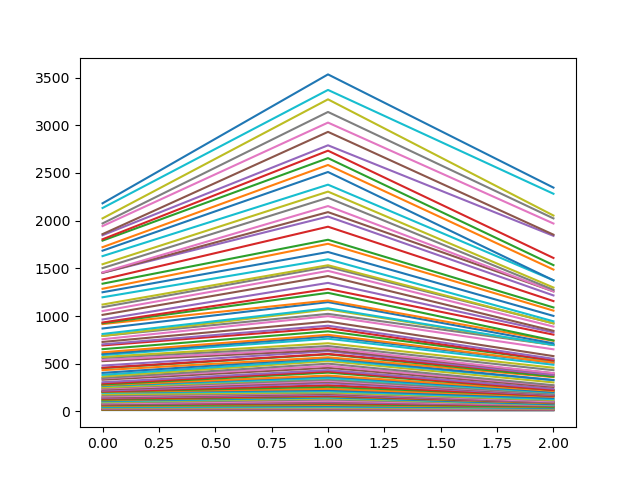
\includegraphics[width=5cm]{wtf}
\caption{wt*.}
\end{figure}



\bibliographystyle{plain} 
\bibliography{ex.bib}
\end{document}
